% Options for packages loaded elsewhere
\PassOptionsToPackage{unicode}{hyperref}
\PassOptionsToPackage{hyphens}{url}
%
\documentclass[
]{article}
\usepackage{amsmath,amssymb}
\usepackage{lmodern}
\usepackage{iftex}
\ifPDFTeX
  \usepackage[T1]{fontenc}
  \usepackage[utf8]{inputenc}
  \usepackage{textcomp} % provide euro and other symbols
\else % if luatex or xetex
  \usepackage{unicode-math}
  \defaultfontfeatures{Scale=MatchLowercase}
  \defaultfontfeatures[\rmfamily]{Ligatures=TeX,Scale=1}
\fi
% Use upquote if available, for straight quotes in verbatim environments
\IfFileExists{upquote.sty}{\usepackage{upquote}}{}
\IfFileExists{microtype.sty}{% use microtype if available
  \usepackage[]{microtype}
  \UseMicrotypeSet[protrusion]{basicmath} % disable protrusion for tt fonts
}{}
\makeatletter
\@ifundefined{KOMAClassName}{% if non-KOMA class
  \IfFileExists{parskip.sty}{%
    \usepackage{parskip}
  }{% else
    \setlength{\parindent}{0pt}
    \setlength{\parskip}{6pt plus 2pt minus 1pt}}
}{% if KOMA class
  \KOMAoptions{parskip=half}}
\makeatother
\usepackage{xcolor}
\IfFileExists{xurl.sty}{\usepackage{xurl}}{} % add URL line breaks if available
\IfFileExists{bookmark.sty}{\usepackage{bookmark}}{\usepackage{hyperref}}
\hypersetup{
  pdftitle={Managing emergent recovery dynamics in at-risk metapopulations},
  hidelinks,
  pdfcreator={LaTeX via pandoc}}
\urlstyle{same} % disable monospaced font for URLs
\usepackage[margin=0.75in]{geometry}
\usepackage{color}
\usepackage{fancyvrb}
\newcommand{\VerbBar}{|}
\newcommand{\VERB}{\Verb[commandchars=\\\{\}]}
\DefineVerbatimEnvironment{Highlighting}{Verbatim}{commandchars=\\\{\}}
% Add ',fontsize=\small' for more characters per line
\usepackage{framed}
\definecolor{shadecolor}{RGB}{248,248,248}
\newenvironment{Shaded}{\begin{snugshade}}{\end{snugshade}}
\newcommand{\AlertTok}[1]{\textcolor[rgb]{0.94,0.16,0.16}{#1}}
\newcommand{\AnnotationTok}[1]{\textcolor[rgb]{0.56,0.35,0.01}{\textbf{\textit{#1}}}}
\newcommand{\AttributeTok}[1]{\textcolor[rgb]{0.77,0.63,0.00}{#1}}
\newcommand{\BaseNTok}[1]{\textcolor[rgb]{0.00,0.00,0.81}{#1}}
\newcommand{\BuiltInTok}[1]{#1}
\newcommand{\CharTok}[1]{\textcolor[rgb]{0.31,0.60,0.02}{#1}}
\newcommand{\CommentTok}[1]{\textcolor[rgb]{0.56,0.35,0.01}{\textit{#1}}}
\newcommand{\CommentVarTok}[1]{\textcolor[rgb]{0.56,0.35,0.01}{\textbf{\textit{#1}}}}
\newcommand{\ConstantTok}[1]{\textcolor[rgb]{0.00,0.00,0.00}{#1}}
\newcommand{\ControlFlowTok}[1]{\textcolor[rgb]{0.13,0.29,0.53}{\textbf{#1}}}
\newcommand{\DataTypeTok}[1]{\textcolor[rgb]{0.13,0.29,0.53}{#1}}
\newcommand{\DecValTok}[1]{\textcolor[rgb]{0.00,0.00,0.81}{#1}}
\newcommand{\DocumentationTok}[1]{\textcolor[rgb]{0.56,0.35,0.01}{\textbf{\textit{#1}}}}
\newcommand{\ErrorTok}[1]{\textcolor[rgb]{0.64,0.00,0.00}{\textbf{#1}}}
\newcommand{\ExtensionTok}[1]{#1}
\newcommand{\FloatTok}[1]{\textcolor[rgb]{0.00,0.00,0.81}{#1}}
\newcommand{\FunctionTok}[1]{\textcolor[rgb]{0.00,0.00,0.00}{#1}}
\newcommand{\ImportTok}[1]{#1}
\newcommand{\InformationTok}[1]{\textcolor[rgb]{0.56,0.35,0.01}{\textbf{\textit{#1}}}}
\newcommand{\KeywordTok}[1]{\textcolor[rgb]{0.13,0.29,0.53}{\textbf{#1}}}
\newcommand{\NormalTok}[1]{#1}
\newcommand{\OperatorTok}[1]{\textcolor[rgb]{0.81,0.36,0.00}{\textbf{#1}}}
\newcommand{\OtherTok}[1]{\textcolor[rgb]{0.56,0.35,0.01}{#1}}
\newcommand{\PreprocessorTok}[1]{\textcolor[rgb]{0.56,0.35,0.01}{\textit{#1}}}
\newcommand{\RegionMarkerTok}[1]{#1}
\newcommand{\SpecialCharTok}[1]{\textcolor[rgb]{0.00,0.00,0.00}{#1}}
\newcommand{\SpecialStringTok}[1]{\textcolor[rgb]{0.31,0.60,0.02}{#1}}
\newcommand{\StringTok}[1]{\textcolor[rgb]{0.31,0.60,0.02}{#1}}
\newcommand{\VariableTok}[1]{\textcolor[rgb]{0.00,0.00,0.00}{#1}}
\newcommand{\VerbatimStringTok}[1]{\textcolor[rgb]{0.31,0.60,0.02}{#1}}
\newcommand{\WarningTok}[1]{\textcolor[rgb]{0.56,0.35,0.01}{\textbf{\textit{#1}}}}
\usepackage{graphicx}
\makeatletter
\def\maxwidth{\ifdim\Gin@nat@width>\linewidth\linewidth\else\Gin@nat@width\fi}
\def\maxheight{\ifdim\Gin@nat@height>\textheight\textheight\else\Gin@nat@height\fi}
\makeatother
% Scale images if necessary, so that they will not overflow the page
% margins by default, and it is still possible to overwrite the defaults
% using explicit options in \includegraphics[width, height, ...]{}
\setkeys{Gin}{width=\maxwidth,height=\maxheight,keepaspectratio}
% Set default figure placement to htbp
\makeatletter
\def\fps@figure{htbp}
\makeatother
\setlength{\emergencystretch}{3em} % prevent overfull lines
\providecommand{\tightlist}{%
  \setlength{\itemsep}{0pt}\setlength{\parskip}{0pt}}
\setcounter{secnumdepth}{-\maxdimen} % remove section numbering
\newlength{\cslhangindent}
\setlength{\cslhangindent}{1.5em}
\newlength{\csllabelwidth}
\setlength{\csllabelwidth}{3em}
\newlength{\cslentryspacingunit} % times entry-spacing
\setlength{\cslentryspacingunit}{\parskip}
\newenvironment{CSLReferences}[2] % #1 hanging-ident, #2 entry spacing
 {% don't indent paragraphs
  \setlength{\parindent}{0pt}
  % turn on hanging indent if param 1 is 1
  \ifodd #1
  \let\oldpar\par
  \def\par{\hangindent=\cslhangindent\oldpar}
  \fi
  % set entry spacing
  \setlength{\parskip}{#2\cslentryspacingunit}
 }%
 {}
\usepackage{calc}
\newcommand{\CSLBlock}[1]{#1\hfill\break}
\newcommand{\CSLLeftMargin}[1]{\parbox[t]{\csllabelwidth}{#1}}
\newcommand{\CSLRightInline}[1]{\parbox[t]{\linewidth - \csllabelwidth}{#1}\break}
\newcommand{\CSLIndent}[1]{\hspace{\cslhangindent}#1}
\usepackage{setspace}
\singlespacing
\usepackage{wrapfig}
\usepackage{lipsum}
\usepackage{float}
\usepackage{lineno}
\usepackage{amsmath}
\linenumbers
\renewcommand{\thefigure}{S\arabic{figure}}
\renewcommand{\thetable}{S\arabic{table}}
\renewcommand{\theequation}{S.\arabic{equation}}
\usepackage{fancyhdr}
\setlength{\parskip}{\baselineskip}
\usepackage{tocloft}
\setlength{\cftbeforesecskip}{6pt}
\ifLuaTeX
  \usepackage{selnolig}  % disable illegal ligatures
\fi

\title{Managing emergent recovery dynamics in at-risk metapopulations}
\usepackage{etoolbox}
\makeatletter
\providecommand{\subtitle}[1]{% add subtitle to \maketitle
  \apptocmd{\@title}{\par {\large #1 \par}}{}{}
}
\makeatother
\subtitle{Supplemental materials: Model details \& results}
\author{Kyle L. Wilson\(^\textup{1,2}\)\footnote{Corresponding author -
  email:
  \href{mailto:klwilson.ccira@gmail.com}{\nolinkurl{klwilson.ccira@gmail.com}}},
Alexandra C. Sawyer\(^\textup{1}\), Anna Potapova\(^\textup{1}\), Colin
J. Bailey\(^\textup{1}\),Daniella LoScerbo\(^\textup{3,4}\),\\
Elissa K. Sweeney-Bergen\(^\textup{1,5}\), Emma E.
Hodgson\(^\textup{1,4}\), Kara J. Pitman\(^\textup{1}\), Karl M.
Seitz\(^\textup{1}\),\\
Lauren Law\(^\textup{1,6}\), Luke Warkentin\(^\textup{1,7}\), Samantha
M. Wilson\(^\textup{1}\), William I. Atlas\(^\textup{1,8}\),\\
Douglas C. Braun\(^\textup{3,5}\), Matthew R. Sloat\(^\textup{8}\), M.
Tim Tinker\(^\textup{9}\),\\
and Jonathan W. Moore\(^\textup{1,3}\)\\
\strut \\
\(^\textup{1}\)Earth to Ocean Research Group, Simon Fraser University\\
\(^\textup{2}\)Central Coast Indigenous Resource Alliance, Campbell
River, BC\\
\(^\textup{3}\)Resource and Environmental Management, Simon Fraser
University\\
\(^\textup{4}\)Fisheries \& Oceans Canada, Cultus Lake Laboratory,
Cultus Lake, BC\\
\(^\textup{5}\)Ministry of Forests, Lands, Natural Resource Operations,
and Rural Development, Smithers, BC\\
\(^\textup{6}\)Fisheries \& Oceans Canada, Salmonid Enhancement Program,
Nanaimo, BC\\
\(^\textup{7}\)Fisheries \& Oceans Canada, North Coast Stock Assessment,
Smithers, BC\\
\(^\textup{8}\)Wild Salmon Center, Portland, OR\\
\(^\textup{9}\)Ecology and Evolutionary Biology, University of
California Santa Cruz}
\date{12 May 2022}

\begin{document}
\maketitle

\centering
\raggedright
\renewcommand{\baselinestretch}{1}\normalsize
\tableofcontents
\renewcommand{\baselinestretch}{0.75}\normalsize
\newpage

\pagestyle{fancy}
\fancyhead[LO,LE]{Wilson \textit{et al.}}
\fancyhead[RO,RE]{\textbf{Appendix A}: Emergent spatial recoveries}

\hypertarget{metapopulation-model}{%
\subsection{Metapopulation model}\label{metapopulation-model}}

\hypertarget{local-metapopulation-dynamics}{%
\subsubsection{Local \& metapopulation
dynamics}\label{local-metapopulation-dynamics}}

Our metapopulation was defined by a set of \(P\) local populations for a
species with a one year generation time with time-dynamics that follows
birth (i.e., recruitment \emph{R}), immigration, death, and emigration
processes typical to metapopulation theory and tested the role of
multiple spatial, temporal, and density-dependent processes (Anderson et
al. 2015; Okamoto et al. 2020):

\begin{align}
N_{i,t}= R_{i,t}+{\sum\limits_{\substack{j=1 \\ j\neq i}}^{P} \omega p_{i,j}R_{j,t}}-d_{i,t}R_{i,t}-\omega R_{i,t}
\end{align}

where \(N_{i,t}\) was the number of adults in patch \emph{i} at time
\emph{t}, \(R_{i,t}\) was the number of recruits at time \emph{t},
\({\sum\limits_{\substack{j=1 \\ j\neq i}}^{P} \omega p_{i,j}R_{j,t}}\)
was the number of recruits immigrating into patch \emph{i} from any
other patch, \(\omega\) was the proportion of local recruits to
disperse, \(p_{i,j}\) was a distance-dependent dispersal function, and
\(d_{i,t}\) was the proportion of recruits that die due to disturbance
regime.

Local patch recruitment at time \emph{t} depended on adult densities at
\emph{t-1} and followed a reparameterized Beverton-Holt function
(Walters \& Martell 2004; Forrest et al. 2010):

\begin{align}
R_{i,t}=\cfrac{\alpha_iN_{i,t-1}}{1+\cfrac{\alpha_i-1}{\beta_i}N_{i,t-1}}\epsilon_{i,t}
\end{align}

where \(\alpha_i\) was the recruitment compensation ratio, \(\beta_i\)
was local patch carrying capacity, and \(\epsilon_{i,t}\) was
lognormally distributed deviates to introduce stochastic recruitment
dynamics.

Resource monitoring often occurs at the scale of the whole
metapopulation by aggregating abundances among local populations to
(Anderson et al. 2015; Moore et al. 2021), hence we define
metapopulation adults as:

\begin{align}
{A}_t = \sum_{i=1}^{P} N_{i,t}
\end{align}

with metapopulation recruits:

\begin{align}
K_t = \sum_{i=1}^{P} R_{i,t}
\end{align}

Monitoring at the scale of the whole metapopulation can produce
productivity relationships that aggregates the population dynamics and
productivity among all local populations. For example, take a two patch
metapopulation model that varies \(\alpha_i\) and \(\beta_i\) parameters
where:

\begin{Shaded}
\begin{Highlighting}[]
\NormalTok{alpha }\OtherTok{\textless{}{-}} \FunctionTok{c}\NormalTok{(}\DecValTok{2}\NormalTok{, }\DecValTok{4}\NormalTok{)}
\NormalTok{beta }\OtherTok{\textless{}{-}} \FunctionTok{c}\NormalTok{(}\DecValTok{100}\NormalTok{, }\DecValTok{200}\NormalTok{)}
\end{Highlighting}
\end{Shaded}

Here, recruitment compensation from local patches \(\alpha_i\) gets
averaged across the metapopulation leading to an average compensation
ratio \(\bar{\alpha}\) of 3. Likewise, the total carrying capacity of
the metapopulation \(\bar{\beta}\) becomes the summation of local patch
carrying capacities \(\sum\beta_i\), which was 300. This scale of
monitoring generates the following local patch and metapopulation
dynamics:

\begin{figure}[H]

{\centering 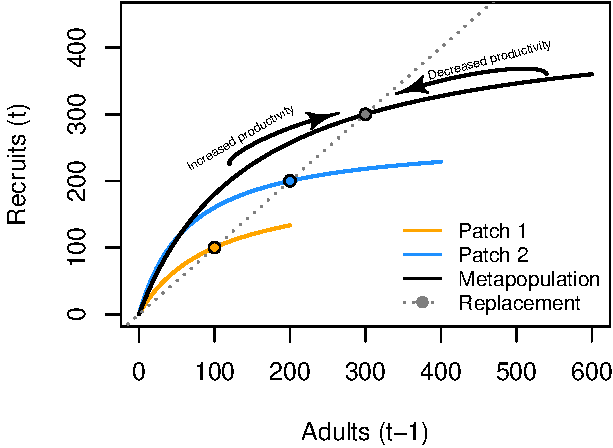
\includegraphics{Managing_for_ecological_surprises_in_metapopulations_files/figure-latex/recruit curves-1} 

}

\caption{Metapopulation and local patch recruitment dynamics.}\label{fig:recruit curves}
\end{figure}

\hypertarget{creating-the-spatial-networks}{%
\subsubsection{Creating the spatial
networks}\label{creating-the-spatial-networks}}

The next aspect to our metapopulation model was connecting the set of
patches to one another (Yeakel et al. 2014). We need to specify the
number of patches, their arrangements (i.e., connections), and how far
apart they are from one another. We followed some classic metapopulation
and source-sink arrangements to create four networks that generalize
across a few real-world topologies: a linear habitat network (e.g.,
coastline), a dendritic or branching network (e.g., coastal rivers), a
star network (e.g., mountain \& valley, or lake with inlet tributaries),
and a grid network (e.g., grasslands).

To make networks comparable, each spatial network type needs the same
leading parameters (e.g., number of patches \(P\) and mean distance
between neighboring patches \(\bar{d}\)). In this case, we set \(P\) to
\texttt{16} and \(\bar{d}\) to \texttt{1} unit (distance units are
arbitrary). We used the \texttt{igraph} package (Csardi \& Nepusz 2006)
and some custom code to arrange our spatial networks as the following:

\begin{figure}[H]

{\centering 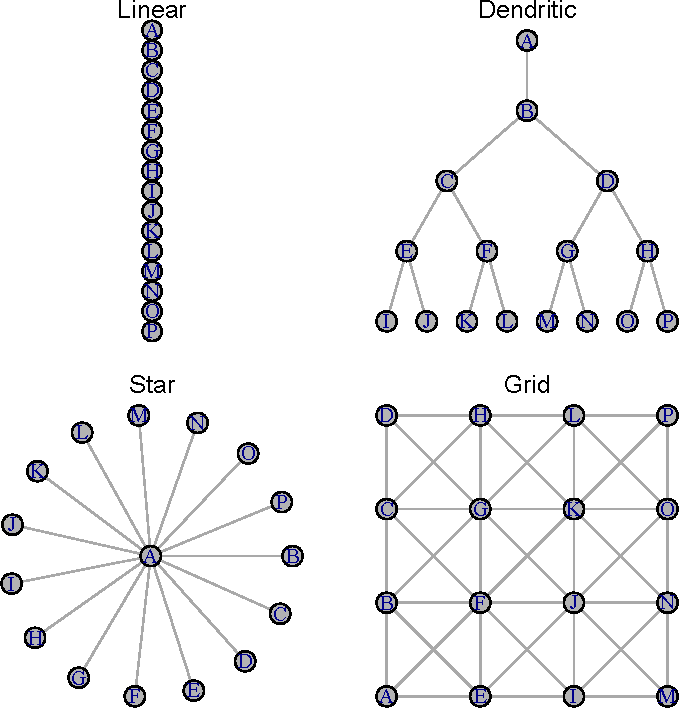
\includegraphics{Managing_for_ecological_surprises_in_metapopulations_files/figure-latex/networks-1} 

}

\caption{Four spatial network topologies.}\label{fig:networks}
\end{figure}

Note that distances between neighbor patches in the above networks are
equal.

\newpage

An example dispersal matrix for the grid network:

\begin{verbatim}
##   A B E F C G D H I J K L M N O P
## A 0 1 1 1 2 2 3 3 2 2 2 3 3 3 3 3
## B 1 0 1 1 1 1 2 2 2 2 2 2 3 3 3 3
## E 1 1 0 1 2 2 3 3 1 1 2 3 2 2 2 3
## F 1 1 1 0 1 1 2 2 1 1 1 2 2 2 2 2
## C 2 1 2 1 0 1 1 1 2 2 2 2 3 3 3 3
## G 2 1 2 1 1 0 1 1 2 1 1 1 2 2 2 2
## D 3 2 3 2 1 1 0 1 3 2 2 2 3 3 3 3
## H 3 2 3 2 1 1 1 0 3 2 1 1 3 2 2 2
## I 2 2 1 1 2 2 3 3 0 1 2 3 1 1 2 3
## J 2 2 1 1 2 1 2 2 1 0 1 2 1 1 1 2
## K 2 2 2 1 2 1 2 1 2 1 0 1 2 1 1 1
## L 3 2 3 2 2 1 2 1 3 2 1 0 3 2 1 1
## M 3 3 2 2 3 2 3 3 1 1 2 3 0 1 2 3
## N 3 3 2 2 3 2 3 2 1 1 1 2 1 0 1 2
## O 3 3 2 2 3 2 3 2 2 1 1 1 2 1 0 1
## P 3 3 3 2 3 2 3 2 3 2 1 1 3 2 1 0
\end{verbatim}

\hypertarget{dispersal}{%
\subsubsection{Dispersal}\label{dispersal}}

Dispersal from patch \emph{i} into patch \emph{j} depends on constant
dispersal rate \(\omega\) (defined as the proportion of total local
recruits that will disperse) and an exponential distance-decay function
between \emph{i} and \emph{j} with distance cost to dispersal \(m\)
following Anderson et al. (2015):

\begin{align}
E_{i,j,t}=\omega R_{i,t}p_{i,j}
\end{align}

where \(E_{i,j}\) was the total dispersing animals from patch \emph{i}
into patch \emph{j} resulting from dispersal rate \(\omega\), total
number of local recruits \(R_{i,t}\), and probability of dispersal
between patches \(p_{i,j}\):

\begin{align}
p_{i,j}=\dfrac{e^{-md_{i,j}}}{\sum\limits_{\substack{j=1 \\ j\neq i}}^{P} e^{-md_{i,j}}}
\end{align}

where \(d_{i,j}\) was the pairwise distance between patches, \(m\) was
the distance cost to dispersal. The summation term in the denominator
normalizes the probability of moving to any patch to between 0 and 1
with the constraint that dispersers cannot move back into their home
patch (i.e., \(j\neq i\). With \(\bar{d}= 1\), \(m=0.5\),
\(\omega=0.1\), \(R_{i,t}=100\) in a linear network):

\begin{figure}[H]

{\centering 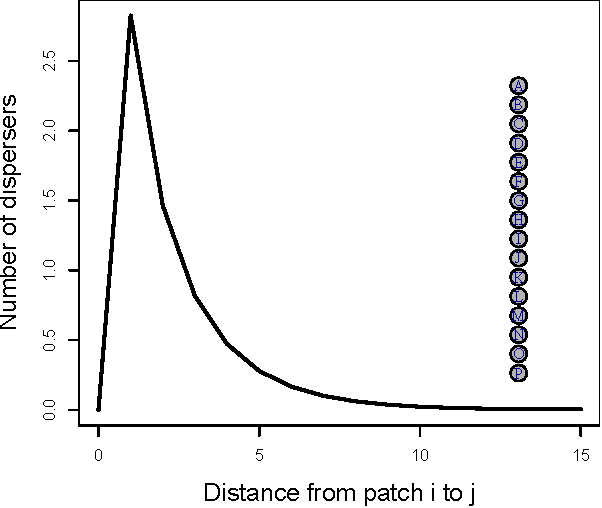
\includegraphics{Managing_for_ecological_surprises_in_metapopulations_files/figure-latex/dispersal-1} 

}

\caption{Example dispersal patterns across linear network.}\label{fig:dispersal}
\end{figure}

\hypertarget{disturbance-regimes}{%
\subsubsection{Disturbance regimes}\label{disturbance-regimes}}

In all scenarios, disturbance was applied after \texttt{50} years of
equilibrating the metapopulation at pristine conditions. We then applied
the disturbance regime at year \texttt{50} (the regime varied from
\emph{uniform}, \emph{localized, even}, and \emph{localized, uneven} -
see \emph{Scenarios} below). Disturbance immediately removed a fixed
proportion of the metapopulation adults at that time (i.e., \texttt{0.9}
of \(A_{t=50}\)). Once applied, the metapopulation was no longer
disturbed and spatio-temporal recovery dynamics emerged from these
conditions given the ecological scenarios of network complexity,
dispersal rate, spatio-temporal correlations, local patch demographies,
and magnitude of stochastic variance.

\begin{figure}[H]

{\centering 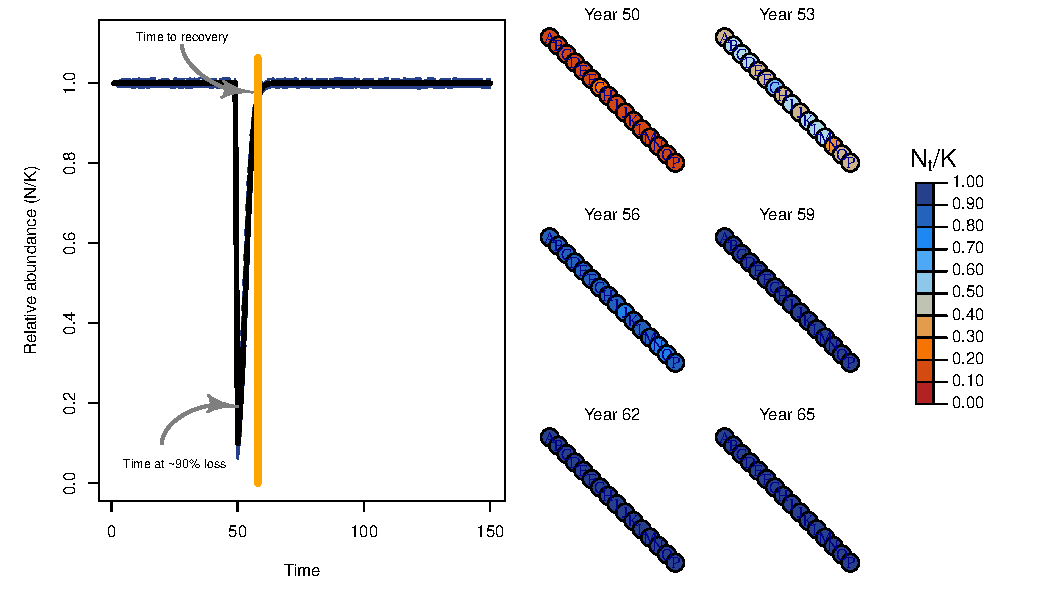
\includegraphics{Managing_for_ecological_surprises_in_metapopulations_files/figure-latex/example disturbance regime-1} 

}

\caption{Recovery regime of metapopulation with linear topology through time (a) and space (b).}\label{fig:example disturbance regime}
\end{figure}

\hypertarget{recruitment-stochasticity}{%
\subsubsection{Recruitment
stochasticity}\label{recruitment-stochasticity}}

Our model allowed for stochastic recruitment that followed a lognormal
distribution with average variation in recruitment of \(\sigma_R\). In
cases with stochastic recruitment, the deterministic recruitment in eq.
S.4 becomes:

\begin{align}
R_{i,t}=\cfrac{\alpha_iN_{i,t-1}}{1+\cfrac{\alpha_i-1}{\beta_i}N_{i,t-1}}e^{(\epsilon_{i,t}-\cfrac{\sigma_{R}^2}{2})}
\end{align}

where lognormal deviates for each patch \emph{i} at time \emph{t} were
drawn from a multivariate normal distribution (\emph{MVN}) with bias
correction \(\cfrac{\sigma_{R}^2}{2}\). If \(\sigma_R\) was low, then
metapopulation dynamics approach the deterministic case. In some
scenarios, we evaluated the role of spatially and/or temporally
correlated deviates among local patches to model potential common
drivers affecting metapopulation dynamics (e.g., Moran effects).
Expected recruitment deviates followed a first-order autoregression
model such that:

\begin{align}
\epsilon_{i,t}=\rho_T\epsilon_{t-1}+MVN(\mu=0,\Sigma=\sigma_R^2(1-\rho_T^2)e^{(-\rho_SD_{i,j})})
\end{align}

where \(\rho_T\) was temporal correlation (bounded \(0-1\)) \(\rho_S\)
was rate of distance-decay in spatial correlation (bounded \(0-\infty\)
with higher values leading to independent patches). If \(\rho_T\) was 0
and \(\rho_S\) was high, then annual recruitment deviates were
independent. We modelled the initial conditions for autoregressive
recruitment deviates \(\epsilon_{i,1}\) by drawing from a stationary
normal distribution with mean \(\mu=0\) and variance \(\sigma_R^2\) such
that: \begin{align}
\epsilon_{i,1} \sim N(\mu=0,\sigma=\sigma_R)
\end{align} We illustrate the effects of four kinds of recruitment
deviates below using the same random number generator seed:

\begin{figure}[H]

{\centering 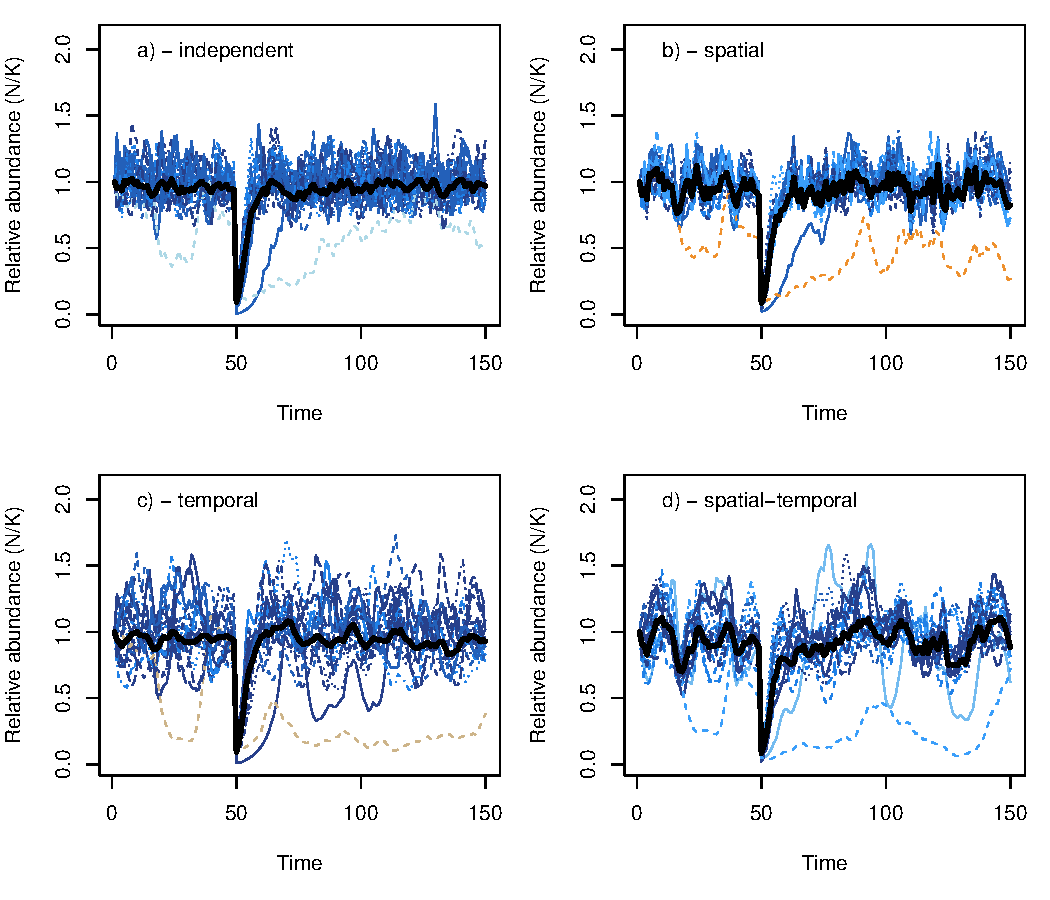
\includegraphics{Managing_for_ecological_surprises_in_metapopulations_files/figure-latex/independent stochasticity-1} 

}

\caption{Metapopulation dynamics with independent (a), spatially correlated (b), temporally correlated (c), and spatio-temporally correlated (d) recruitment deviates. Black line indicates metapopulation, and dashed lines indicate local patches with red and blue relating to abundances after 100 years post-disturbance were less than or greater than 1.0 pre-disturbance, respectively.}\label{fig:independent stochasticity}
\end{figure}

\hypertarget{post-disturbance-outcomes}{%
\subsection{Post-disturbance outcomes}\label{post-disturbance-outcomes}}

We measured the following post-disturbance outcomes to track the
temporal and spatial recovery regime of the metapopulation.

\begin{enumerate}
\def\labelenumi{\arabic{enumi}.}
\item
  Non-recovery (a) \& recovery rate (b) after disturbance:

  \begin{enumerate}
  \def\labelenumii{\alph{enumii}.}
  \tightlist
  \item
    Non-recovery rate was defined as the \% of simulations where
    metapopulation abundance failed to recover to \texttt{1.0} of the
    average pre-disturbance abundance for \texttt{5} consecutive years
    post-disturbance. This ``non-recovery rate'' reflects the risk of a
    long-term state shift in metapopulation dynamics after disturbance
    in the face of stochasticity.
  \item
    Recovery rate represents the proportional post-disturbance recovery
    towards metapopulation carrying capacity gained per year (1 year = 1
    generation in our models). Recovery rate was calculated as
    \(1-T_{recovery}/T_{sim}\) where the recovery time,
    \(T_{recovery}\), was the number of years/generations it took for
    the metapopulation to reach five consecutive years ≥ pre-disturbance
    abundance. Recovery rate captures how quickly the aggregate
    metapopulation recovers from disturbance but doesn't take into
    account whether any given local patches recover to their
    pre-disturbance capacity nor did it allow for any uncertainty around
    recovery criteria.
  \end{enumerate}
\item
  Patch occupancy - the mean number of patches with
  \texttt{\textgreater{}0.1} local carrying capacity after disturbance
  in the short-term (5 years), medium-term (10 years), and long-term (25
  years). This value characterizes the expected risk of spatial
  contractions or local patch collapses, and reflects how interactions
  between spatial structure, disturbance, and dispersal shape
  source-sink dynamics and the ability to provide (or not) rescue
  effects and recover local patches.
\item
  The ratio of expected maximum surplus production (we term \emph{MSY})
  to true maximum surplus production summed across all patches from
  fitted stock-recruitment model to aggregate across metapopulation such
  that:\\
  \begin{align}
  \Delta_{MSY}=\cfrac{\hat{MSY_M}}{\sum_{i=1}^{P} MSY_{i}}
  \end{align}\\
  A value of 1.0 would indicate that the disturbed metapopulation can
  sustain itself against the same disturbance regime as the sum of each
  patch independently. In other words, was the metapopulation more than
  (\(\Delta_{MSY}\)\textgreater1.0), less than
  (\(\Delta_{MSY}\)\textless1.0), or equal to the sum of its parts
  (\(\Delta_{MSY}\)=1.0). We detail how \emph{MSY} was estimated further
  below.
\end{enumerate}

\hypertarget{monitoring-management-at-aggregate-scale}{%
\subsubsection{Monitoring \& management at
aggregate-scale}\label{monitoring-management-at-aggregate-scale}}

While true metapopulation dynamics emerge from local patch dynamics and
dispersal in S.1, natural resource managers often monitor and manage at
the scale of the metapopulation. Hence, management at this scale
inherently defines the stock-recruitment dynamics of the aggregate
complex of patches (i.e., metapopulation) as:

\begin{align}
{K}_{t}=\cfrac{\hat{\alpha_t}{A}_{t-1}}{1+\cfrac{\hat{\alpha_t}-1}{\hat{\beta_t}}{A}_{i,t-1}}
\end{align}

where \(\hat{\alpha_t}\) was the estimated compensation ratio averaged
across the metapopulation at time \emph{t} and \(\hat{\beta_t}\) was the
estimated carrying capacity of the entire metapopulation. Necessarily,
these estimates emerge from monitoring data collected across all patches
and are sensitive to the quality of the data and how local patches
perform through time. For example, temporal shifts in productivity
regimes may be masked if most of the data were sampled before the regime
shift. To help surmount these issues, modern resource assessments use
data weighting and penalties (i.e., priors) when fitting models to data.

In our assessment, we weighted recent years of sampling over more
distant years such that:

\begin{figure}[H]

{\centering 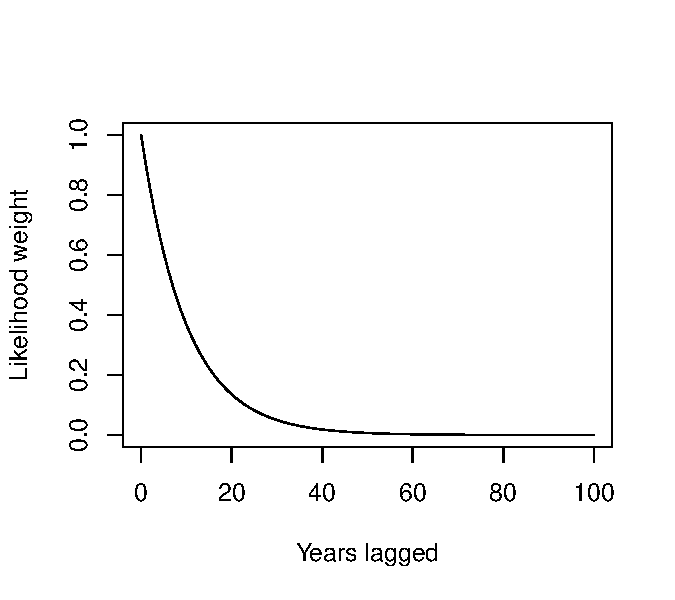
\includegraphics{Managing_for_ecological_surprises_in_metapopulations_files/figure-latex/unnamed-chunk-1-1} 

}

\caption{Likelihood weighting for samples collected over time from current year of sampling.}\label{fig:unnamed-chunk-1}
\end{figure}

This forward-weighting approach increased the sensitivity of the
monitoring sub-model to detect demographic changes in the
post-disturbance recovery regime. Data-weighting is increasingly being
used in resource monitoring, although how weights are developed and
applied to data is a case-by-case basis.

Furthermore, we used penalized normal likelihoods on both
\(\hat{\alpha_t}\) and \(\hat{\beta_t}\) such that:

\begin{align}
\hat{\alpha_t} \sim N(\mu=\hat{\alpha_{t-1}},\sigma=3\hat{\alpha_{t-1}})
\end{align}

and

\begin{align}
\hat{\beta_t} \sim N(\mu=\hat{\beta_{t-1}},\sigma=3\hat{\beta_{t-1}})
\end{align}

where \(\mu=\hat{\alpha_{t-1}}\) and \(\mu=\hat{\beta_{t-1}}\)
represents the best estimates from the previous assessment and the
\texttt{3} in the \(\sigma\) term represents a 300\% coefficient of
variation. We used these penalized likelihoods to fit the above
aggregate stock-recruitment model with \emph{lognormal} error to the
metapopulation stock-recruit data collected at time \emph{t}. We used
the following function and fitted to the below \(\theta\) parameters
(termed \texttt{theta} in the function \texttt{optim()} using the
\texttt{L-BFGS-B} optimizer with a lower bound on \(\hat{\alpha}\) of
\texttt{1.01} (i.e., constrained to be at least above replacement).

\begin{Shaded}
\begin{Highlighting}[]
\NormalTok{SRfn }\OtherTok{\textless{}{-}} \ControlFlowTok{function}\NormalTok{(theta, data, lastYr) \{}
\NormalTok{    a.hat }\OtherTok{\textless{}{-}}\NormalTok{ theta[}\DecValTok{1}\NormalTok{]}
\NormalTok{    b.hat }\OtherTok{\textless{}{-}} \FunctionTok{exp}\NormalTok{(theta[}\DecValTok{2}\NormalTok{])}
\NormalTok{    sd.hat }\OtherTok{\textless{}{-}} \FunctionTok{exp}\NormalTok{(theta[}\DecValTok{3}\NormalTok{])}
\NormalTok{    rec.mean }\OtherTok{\textless{}{-}}\NormalTok{ (a.hat }\SpecialCharTok{*}\NormalTok{ data}\SpecialCharTok{$}\NormalTok{spawners)}\SpecialCharTok{/}\NormalTok{(}\DecValTok{1} \SpecialCharTok{+}\NormalTok{ ((a.hat }\SpecialCharTok{{-}} \DecValTok{1}\NormalTok{)}\SpecialCharTok{/}\NormalTok{b.hat) }\SpecialCharTok{*}\NormalTok{ data}\SpecialCharTok{$}\NormalTok{spawners)}
    \CommentTok{\# negative log likelihood on recruitment parameters}
\NormalTok{    nll }\OtherTok{\textless{}{-}} \SpecialCharTok{{-}}\DecValTok{1} \SpecialCharTok{*} \FunctionTok{sum}\NormalTok{(}\FunctionTok{dlnorm}\NormalTok{(data}\SpecialCharTok{$}\NormalTok{recruits, }\AttributeTok{meanlog =} \FunctionTok{log}\NormalTok{(rec.mean), }\AttributeTok{sdlog =}\NormalTok{ sd.hat,}
        \AttributeTok{log =} \ConstantTok{TRUE}\NormalTok{) }\SpecialCharTok{*}\NormalTok{ data}\SpecialCharTok{$}\NormalTok{weights, }\AttributeTok{na.rm =} \ConstantTok{TRUE}\NormalTok{)}
    \CommentTok{\# penalized likelihood on estimated alpha}
\NormalTok{    penalty1 }\OtherTok{\textless{}{-}} \SpecialCharTok{{-}}\FunctionTok{dnorm}\NormalTok{(a.hat, lastYr}\SpecialCharTok{$}\NormalTok{alphaLstYr, }\DecValTok{4} \SpecialCharTok{*}\NormalTok{ lastYr}\SpecialCharTok{$}\NormalTok{alphaLstYr, }\AttributeTok{log =} \ConstantTok{TRUE}\NormalTok{)}
    \CommentTok{\# penalized likelihood on estimated carrying capacity}
\NormalTok{    penalty2 }\OtherTok{\textless{}{-}} \SpecialCharTok{{-}}\FunctionTok{dnorm}\NormalTok{(b.hat, lastYr}\SpecialCharTok{$}\NormalTok{metaKLstYr, }\DecValTok{4} \SpecialCharTok{*}\NormalTok{ lastYr}\SpecialCharTok{$}\NormalTok{metaKLstYr, }\AttributeTok{log =} \ConstantTok{TRUE}\NormalTok{)}
\NormalTok{    jnll }\OtherTok{\textless{}{-}} \FunctionTok{sum}\NormalTok{(}\FunctionTok{c}\NormalTok{(nll, penalty1, penalty2), }\AttributeTok{na.rm =} \ConstantTok{TRUE}\NormalTok{)}
    \FunctionTok{return}\NormalTok{(jnll)}
\NormalTok{\}}
\end{Highlighting}
\end{Shaded}

This above function allows us to assess the bias in \(\hat{\alpha_t}\),
\(\hat{\beta_t}\), and \(\hat{K_t}\) compared to true \(\bar{\alpha}\),
\(\bar{\beta}\), and \({K}_t\) across the metapopulation. This then
allows us to see how much information management \& monitoring programs
were missing when they assess metapopulations at the aggregate (rather
than local) scales.

\hypertarget{finding-maximum-sustainable-yield}{%
\subsubsection{Finding maximum sustainable
yield}\label{finding-maximum-sustainable-yield}}

Resource managers measure productivity with a variety of performance
reference points (Forrest et al. 2010). One of the most widely used
metrics, commonly called \emph{Maximum Sustainable Yield} in fisheries
and other harvest literature (\(MSY\)), relates to the largest loss the
population can sustain over an indefinite period of time that maximizes
its ability to replenish itself. Under density-dependent growth,
individuals' growth, survival, and reproduction at low population
densities are not constrained by limited resources, but overall
production is low because there are few individuals. At high densities,
limited resources increasingly constrain individual's reproductive
success until the population reaches carrying capacity, and overall
production drops to zero because per-capita success is low. However, at
some intermediate densities, both per-capita and overall production is
high, and population growth is at its maximum point due to the large
number of reproducing individuals. At this point, there is the maximum
surplus of individuals produced above replacement that can help to
withstand disturbance or harvest regimes and contribute to future
recovery, either through increasing local patch densities or by
emigrating neighboring patches providing ``rescue effects''.

Under Beverton-Holt or Ricker density-dependent recuitment, however,
there exists no analytical solution for calculating \(MSY\). Therefore,
we used numerical methods and a one dimensional root finder to
iteratively search for the population mortality that maximized surplus
production in the metapopulation. We term this mortality \(F_{MSY}\) and
can use this mortality value to calculate maximum surplus production
\(MSY\), the adult densities that produce \(MSY\) (termed \(N_{MSY}\)),
and the recruits that result from this (termed \(R_{MSY}\)).

\begin{Shaded}
\begin{Highlighting}[]
\CommentTok{\# uniroot numerical search}
\NormalTok{yieldRoot }\OtherTok{\textless{}{-}} \ControlFlowTok{function}\NormalTok{(alpha, beta, Fcur, model) \{}
\NormalTok{    Ucur }\OtherTok{\textless{}{-}} \DecValTok{1} \SpecialCharTok{{-}} \FunctionTok{exp}\NormalTok{(}\SpecialCharTok{{-}}\NormalTok{Fcur)}
    \ControlFlowTok{if}\NormalTok{ (model }\SpecialCharTok{==} \StringTok{"Beverton{-}Holt"}\NormalTok{) \{}
        \CommentTok{\# population model is R \textasciitilde{} (CR * S)/(1+(CR{-}1)/K * S): reparameterized}
        \CommentTok{\# Beverton{-}Holt}
\NormalTok{        adults }\OtherTok{\textless{}{-}}\NormalTok{ beta }\SpecialCharTok{*} \FunctionTok{exp}\NormalTok{(}\SpecialCharTok{{-}}\NormalTok{Fcur)}
\NormalTok{        recruits }\OtherTok{\textless{}{-}}\NormalTok{ (alpha }\SpecialCharTok{*}\NormalTok{ adults)}\SpecialCharTok{/}\NormalTok{(}\DecValTok{1} \SpecialCharTok{+}\NormalTok{ ((alpha }\SpecialCharTok{{-}} \DecValTok{1}\NormalTok{)}\SpecialCharTok{/}\NormalTok{beta) }\SpecialCharTok{*}\NormalTok{ adults)}
\NormalTok{        yield }\OtherTok{\textless{}{-}}\NormalTok{ recruits }\SpecialCharTok{{-}}\NormalTok{ adults}
\NormalTok{    \}}
    \ControlFlowTok{if}\NormalTok{ (model }\SpecialCharTok{==} \StringTok{"Ricker"}\NormalTok{) \{}
        \CommentTok{\# population model is R \textasciitilde{} CR * S * e({-}log(CR)/K * S): reparameterized}
        \CommentTok{\# Ricker}
\NormalTok{        adults }\OtherTok{\textless{}{-}}\NormalTok{ beta }\SpecialCharTok{*} \FunctionTok{exp}\NormalTok{(}\SpecialCharTok{{-}}\NormalTok{Fcur)}
\NormalTok{        recruits }\OtherTok{\textless{}{-}}\NormalTok{ alpha }\SpecialCharTok{*}\NormalTok{ adults }\SpecialCharTok{*} \FunctionTok{exp}\NormalTok{((}\SpecialCharTok{{-}}\FunctionTok{log}\NormalTok{(alpha)}\SpecialCharTok{/}\NormalTok{beta) }\SpecialCharTok{*}\NormalTok{ adults)}
\NormalTok{        yield }\OtherTok{\textless{}{-}}\NormalTok{ recruits }\SpecialCharTok{{-}}\NormalTok{ adults}
\NormalTok{    \}}
    \FunctionTok{return}\NormalTok{(}\FunctionTok{list}\NormalTok{(}\AttributeTok{recruits =}\NormalTok{ recruits, }\AttributeTok{adults =}\NormalTok{ adults, }\AttributeTok{yield =}\NormalTok{ yield))}
\NormalTok{\}}

\CommentTok{\# Return approximate gradient for integral}
\NormalTok{fun\_yield }\OtherTok{\textless{}{-}} \ControlFlowTok{function}\NormalTok{(Fcur, alpha, beta, delta, model) \{}
\NormalTok{    y1 }\OtherTok{\textless{}{-}} \FunctionTok{yieldRoot}\NormalTok{(}\AttributeTok{alpha =}\NormalTok{ alpha, }\AttributeTok{beta =}\NormalTok{ beta, }\AttributeTok{Fcur =}\NormalTok{ Fcur }\SpecialCharTok{{-}}\NormalTok{ delta}\SpecialCharTok{/}\DecValTok{2}\NormalTok{, }\AttributeTok{model =}\NormalTok{ model)}\SpecialCharTok{$}\NormalTok{yield}
\NormalTok{    y2 }\OtherTok{\textless{}{-}} \FunctionTok{yieldRoot}\NormalTok{(}\AttributeTok{alpha =}\NormalTok{ alpha, }\AttributeTok{beta =}\NormalTok{ beta, }\AttributeTok{Fcur =}\NormalTok{ Fcur }\SpecialCharTok{+}\NormalTok{ delta}\SpecialCharTok{/}\DecValTok{2}\NormalTok{, }\AttributeTok{model =}\NormalTok{ model)}\SpecialCharTok{$}\NormalTok{yield}
\NormalTok{    approx.gradient }\OtherTok{\textless{}{-}}\NormalTok{ (y2 }\SpecialCharTok{{-}}\NormalTok{ y1)}\SpecialCharTok{/}\NormalTok{delta}
    \FunctionTok{return}\NormalTok{(approx.gradient)}
\NormalTok{\}}

\CommentTok{\# uniroot search for optimal yield and Fmsy}
\NormalTok{findMSY }\OtherTok{\textless{}{-}} \ControlFlowTok{function}\NormalTok{(alpha, beta, Npatches, model) \{}
\NormalTok{    F\_msy }\OtherTok{\textless{}{-}} \ConstantTok{NULL}
    \ControlFlowTok{for}\NormalTok{ (i }\ControlFlowTok{in} \DecValTok{1}\SpecialCharTok{:}\NormalTok{Npatches) \{}
\NormalTok{        a\_p }\OtherTok{\textless{}{-}}\NormalTok{ alpha[i]}
\NormalTok{        b\_p }\OtherTok{\textless{}{-}}\NormalTok{ beta[i]}
\NormalTok{        F\_msy[i] }\OtherTok{\textless{}{-}} \FunctionTok{uniroot}\NormalTok{(fun\_yield, }\AttributeTok{interval =} \FunctionTok{c}\NormalTok{(}\DecValTok{0}\NormalTok{, }\DecValTok{1}\NormalTok{), }\AttributeTok{extendInt =} \StringTok{"yes"}\NormalTok{, }\AttributeTok{alpha =}\NormalTok{ a\_p,}
            \AttributeTok{beta =}\NormalTok{ b\_p, }\AttributeTok{delta =} \FloatTok{1e{-}04}\NormalTok{, }\AttributeTok{model =}\NormalTok{ model)}\SpecialCharTok{$}\NormalTok{root}
\NormalTok{    \}}
\NormalTok{    MSY }\OtherTok{\textless{}{-}} \FunctionTok{sapply}\NormalTok{(}\DecValTok{1}\SpecialCharTok{:}\NormalTok{Npatches, }\ControlFlowTok{function}\NormalTok{(x) \{}
        \FunctionTok{yieldRoot}\NormalTok{(}\AttributeTok{alpha =}\NormalTok{ alpha[x], }\AttributeTok{beta =}\NormalTok{ beta[x], }\AttributeTok{Fcur =}\NormalTok{ F\_msy[[x]][}\DecValTok{1}\NormalTok{], }\AttributeTok{model =}\NormalTok{ model)}
\NormalTok{    \})}
    \FunctionTok{return}\NormalTok{(}\FunctionTok{list}\NormalTok{(}\AttributeTok{F\_msy =}\NormalTok{ F\_msy, }\AttributeTok{MSY =}\NormalTok{ MSY))}
\NormalTok{\}}
\end{Highlighting}
\end{Shaded}

\hypertarget{scenarios}{%
\subsection{Scenarios}\label{scenarios}}

We tested all combinations of the following eight processes (below) and
ran \texttt{100} iterations per scenario to estimate the mean for each
of the above outcomes.

\begin{enumerate}
\def\labelenumi{\arabic{enumi}.}
\item
  Homogenous and spatially variable recruitment compensation ratio
  across patches, i.e.~intrinsic rate of population growth
  (\(\alpha_i\)).
\item
  Homogenous and spatially variable local carrying capacity across
  patches, i.e.~asymptote of expected recruits at high adult densities
  (\(\beta_i\))
\item
  Disturbances where a proportion of individuals removed from
  metapopulation (e.g., \texttt{0.90}) occurs.

  \begin{enumerate}
  \def\labelenumii{\alph{enumii}.}
  \tightlist
  \item
    \emph{uniform} - random individuals removed at equal vulnerability
    across all patches.
  \item
    \emph{localized, even} - random individuals removed from randomly
    selected subset of patches (as long as the target individuals lost
    in the metapopulation can be achieved in that subset of patches)
  \item
    \emph{localized, uneven} - total extirpation of randomly selected
    subset of patches (as long as the target individuals lost in the
    metapopulation can be achieved in that subset of patches)
  \end{enumerate}
\item
  Density-independent dispersal rates \(\omega\) from 0 to 5\% of
  individuals within a patch will disperse.
\item
  Topology of the spatial networks with linear, dendritic, star, and
  grid networks. Each network with \(P=16\) and distance between patches
  \(\bar{d}=1\).
\item
  Stochastic recruitment deviates from low, medium, high coefficient of
  variation on lognormal error. Generate stochasticity in time-dynamics
  via random recruitement deviates away from expected.
\item
  Temporal correlation in recruitment deviates from low, medium, high
  correlation (i.e., good year at time \emph{t} begets good year at time
  \emph{t+1}).
\item
  Spatial correlation in recruitment deviates among patches from low,
  medium, to high correlation (i.e., neighboring patches go up or down
  together).
\end{enumerate}

\hypertarget{example-results}{%
\subsubsection{Example results}\label{example-results}}

We demonstrate our metapopulation model with an example outcome for a
linear network composed of \texttt{16} patches, a dispersal rate of
\texttt{0.01} and a high enough dispersal cost such that individuals are
only willing to move to their closest neighboring patches. This limits
the strength of potential rescue effects. For this example, patches
varied in their productivity and carrying capacity but will have
deterministic population dynamics.

\begin{figure}[H]

{\centering 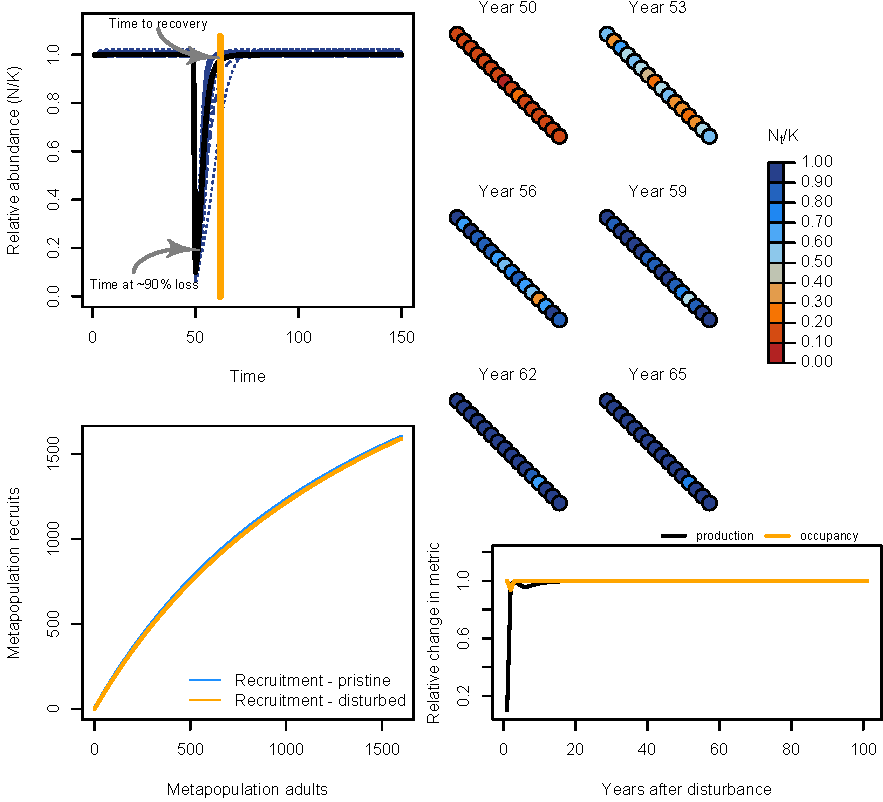
\includegraphics{Managing_for_ecological_surprises_in_metapopulations_files/figure-latex/example results1-1} 

}

\caption{Example iteration of spatial recovery regime of metapopulation with linear topology through time (top left) and space (top right). Recruitment dynamics before and 10 years after disturbance (bottom left). Relative bias in aggregate-scale estimates of carrying capacity, compensation ratio, and recruitment production in recovery phase (bottom right).}\label{fig:example results1}
\end{figure}
\newpage

We can then contrast this with a different network shape, like a
dendritic network.

\begin{figure}[H]

{\centering 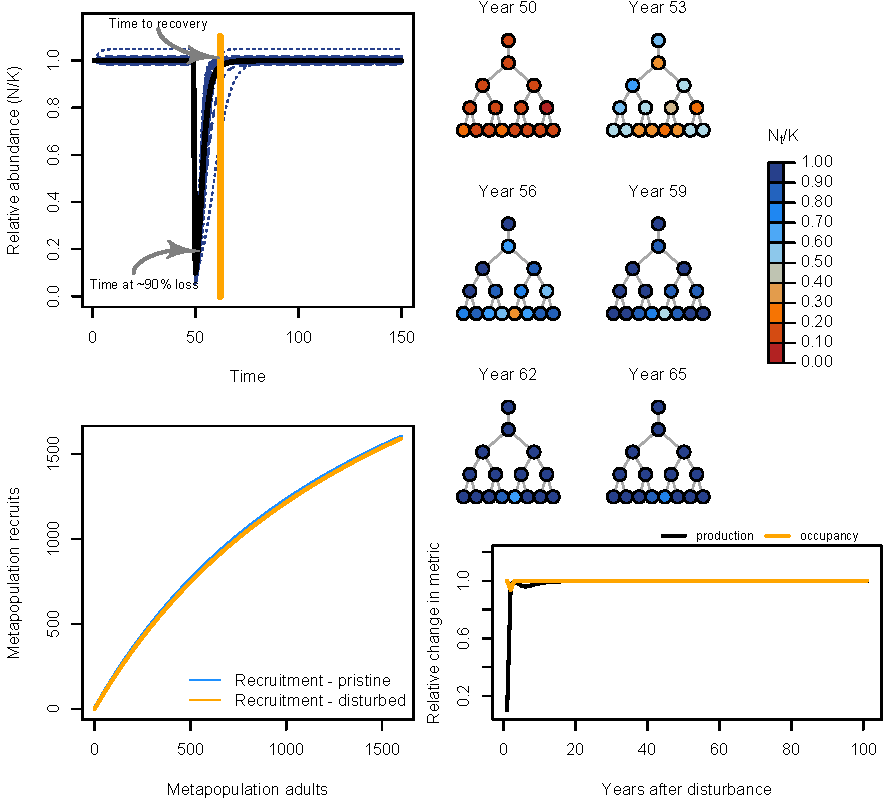
\includegraphics{Managing_for_ecological_surprises_in_metapopulations_files/figure-latex/example results2-1} 

}

\caption{Example iteration of spatial recovery regime of metapopulation with dendritic topology.}\label{fig:example results2}
\end{figure}
\newpage

Now, let's add some stochasticity to recruitment and see how this
affects the recovery regime.

\begin{figure}[H]

{\centering 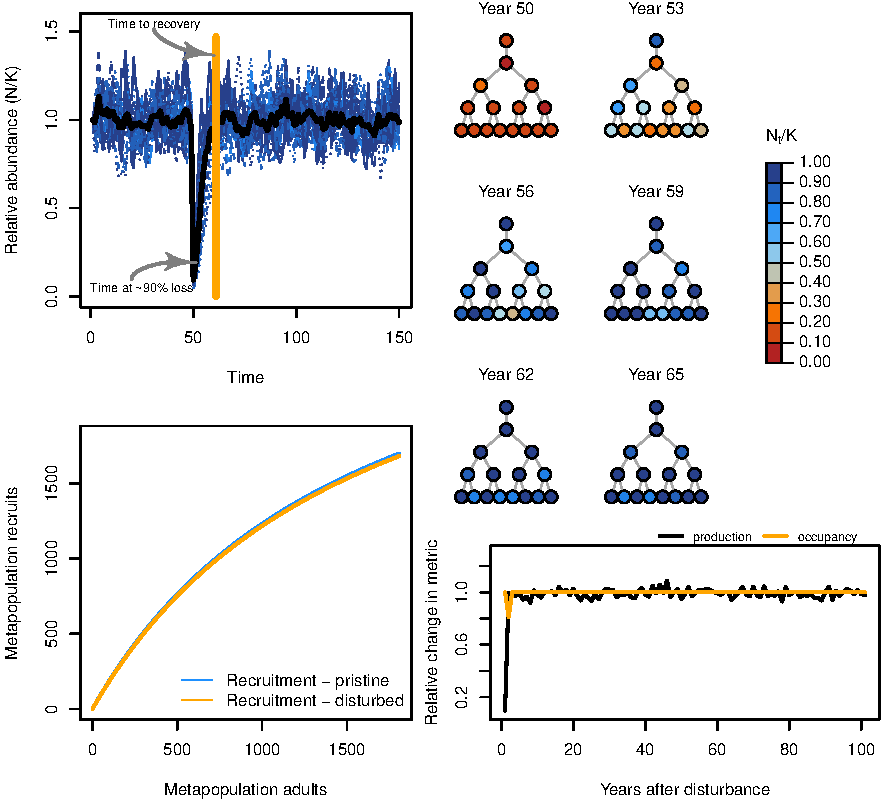
\includegraphics{Managing_for_ecological_surprises_in_metapopulations_files/figure-latex/example results3-1} 

}

\caption{Example iteration of spatial recovery regime of stochastic metapopulation.}\label{fig:example results3}
\end{figure}
\newpage

Next, we can contrast with a disturbance regime where the disturbance is
concentrated on local patches that can be completely extirpated (rather
than the disturbance being applied proportionally across all patches
e.g., a mixed-stock fishery).

\begin{figure}[H]

{\centering 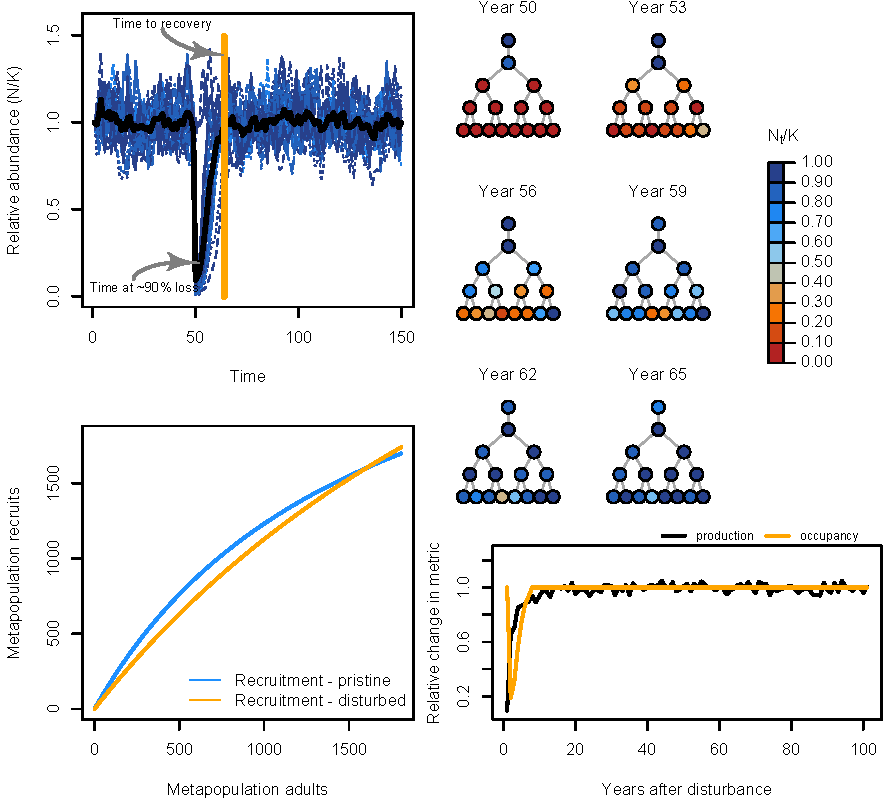
\includegraphics{Managing_for_ecological_surprises_in_metapopulations_files/figure-latex/example results4-1} 

}

\caption{Example iteration of spatial recovery regime of stochastic metapopulation.}\label{fig:example results4}
\end{figure}
\newpage

\hypertarget{general-patterns}{%
\subsection{General patterns}\label{general-patterns}}

\hypertarget{effects-of-disturbance-regime}{%
\subsubsection{Effects of disturbance
regime}\label{effects-of-disturbance-regime}}

The strongest lever influencing recovery in our simulated
metapopulations was, by far, the characteristics of the disturbance
regime. Specifically, the degree to how locally concentrated the
disturbance was on the set of patches was more influential than variable
density dependence, dispersal rates, or network topology. This was
surprising and not expected in our initial hypotheses. Localized
disturbances increased the risk of spatial contraction, reduced recovery
rates and aggregate compensation, and increased the risk of a long-term
state shift. By altering aggregate compensation, localized disturbance
reduced the surplus production of the metapopulation. In other words,
through changes in source-sink dynamics, metapopulations under localized
disturbance acted less than the sum of their parts -- the more localized
the impacts, the worse these effects. Uniform disturbances generally
left the metapopulation dynamics unaffected with few ecological
surprises. These above spatial and temporal recovery processes also
appeared tied to one another such that changes to any of them had
feedbacks with other recovery metrics.

\begin{figure}[H]

{\centering 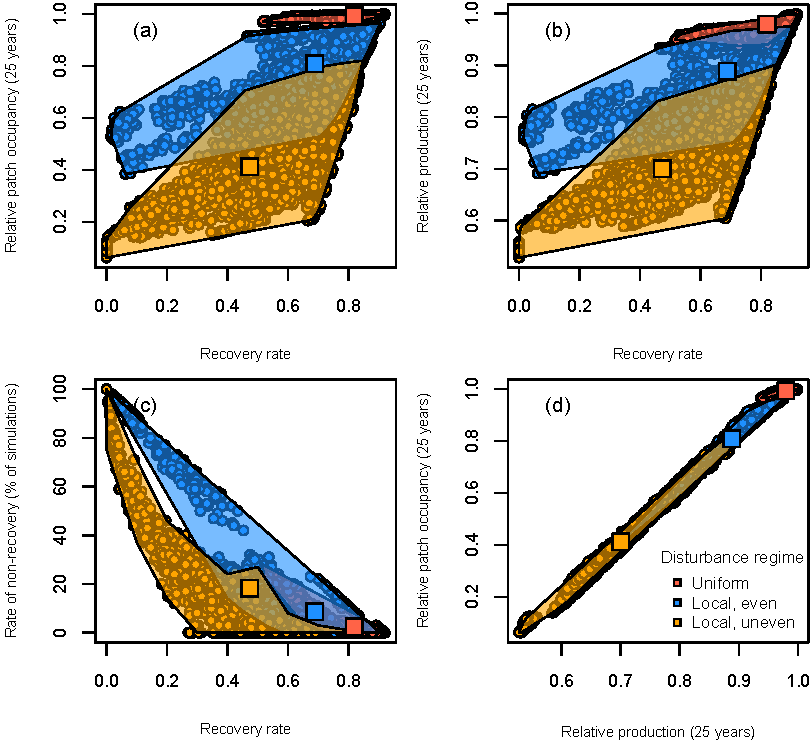
\includegraphics{Managing_for_ecological_surprises_in_metapopulations_files/figure-latex/disturbance regime-1} 

}

\caption{Spatial and temporal recovery patterns along disturbance regimes across all scenarios.}\label{fig:disturbance regime}
\end{figure}
\newpage

\hypertarget{role-of-network-structure-dispersal}{%
\subsubsection{Role of network structure \&
dispersal}\label{role-of-network-structure-dispersal}}

We now show some general patterns in how variable patch demographic
rates, network structure, dispersal, disturbance, recruitment
stochasticity, and spatio-temporal correlations variation affects
metapopulation \emph{recovery rates}, \emph{maximum sustainable yield}
(analagous to the maximum rate of loss the system can sustain), and
\emph{collapse rate} (i.e, the number of simulations where the
metapopulation fails to recover), and \emph{patch occupancy} (i.e.,
number of patches with local abundance \textless10\% of
pre-disturbance).

\begin{figure}[H]

{\centering 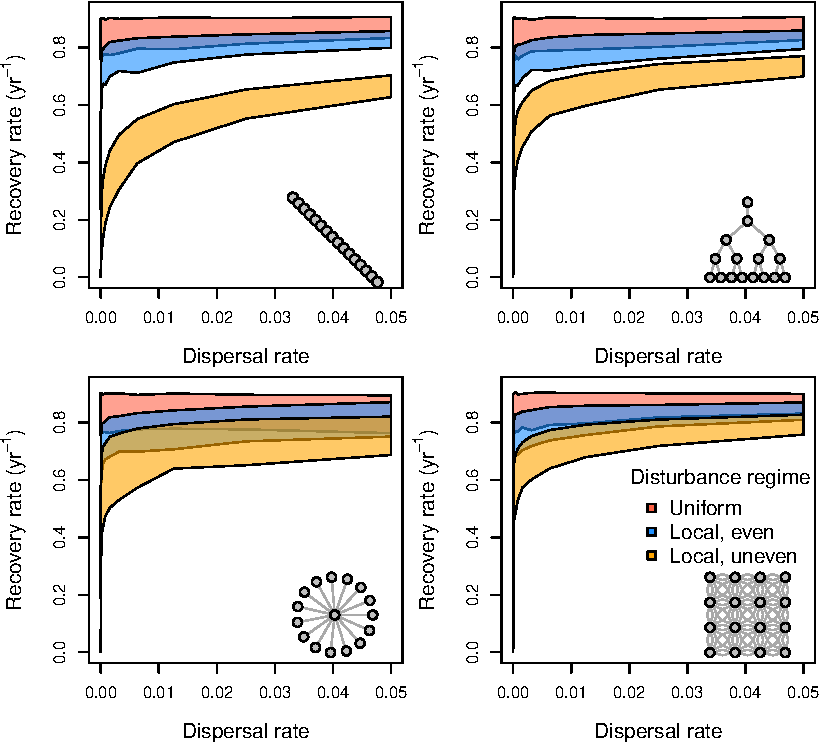
\includegraphics{Managing_for_ecological_surprises_in_metapopulations_files/figure-latex/recovery and dispersal and spatial network-1} 

}

\caption{Metapopulation recovery rates along gradients of network configuration, dispersal rates, and spatial distribution of disturbance. The shaded region describes the interquartile range across all scenarios.}\label{fig:recovery and dispersal and spatial network}
\end{figure}

Dispersal, landscape structure, and local density-dependence also
affected metapopulation recovery patterns in three key ways, though to a
lesser extent. First, recovery rates increased with increased dispersal.
However, this effect was nonlinear with diminishing benefits of
dispersal occurring at \textasciitilde1-3\%, depending on spatial
structure and disturbance. Second, more linearized networks had slower
recovery times than more connected networks suggesting that rescue
effects take some time to cascade through the entire network of patches;
but this interacted with the disturbance regime as only local,
extirpation exhibited this change in any substantial manner. Last,
diversity in local patch compensation and carrying capacities tended to
slow metapopulation recoveries - this effect interacted with other
factors like stochasticity.

\begin{figure}[H]

{\centering 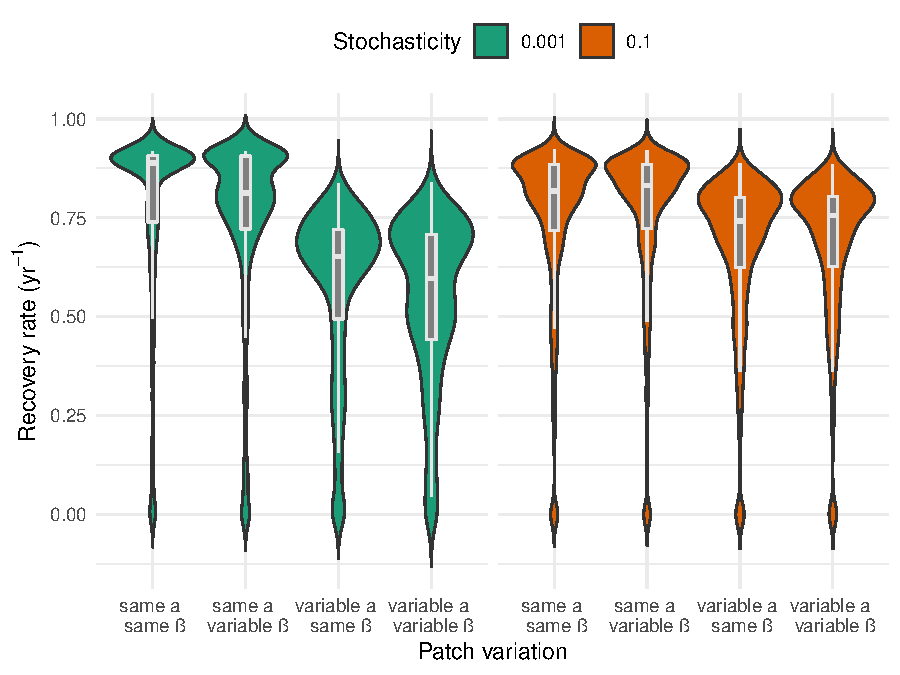
\includegraphics{Managing_for_ecological_surprises_in_metapopulations_files/figure-latex/recovery with patch variation-1} 

}

\caption{Effects of variable local patch productivities on metapopulation recovery across all scenarios.}\label{fig:recovery with patch variation}
\end{figure}
\newpage

\hypertarget{surprising-ecological-outcomes}{%
\subsubsection{Surprising ecological
outcomes}\label{surprising-ecological-outcomes}}

Metapopulation recovery regimes emerged from a complex interplay of
density-dependent productivity (shown in Figure 6 of the main text),
network structure (shown here), dispersal, and disturbance regimes.
Overall, clustering analyses of our model results found evidence for six
common outcomes: (1) resilient recovery -- metapopulation recovery
\textless10 years, (2) slow recovery -- metapopulation recovery
\textgreater10 years and no other surprise, (3) lost capacity --
long-term maximum surplus production \textless50\% before disturbance,
(4) hidden collapses -- metapopulation recovered (or was recovering) but
50\% of patches remain unoccupied, (5) spatial contraction --
\textgreater25\% of patches remain unoccupied and (6) critical risk --
metapopulation abundance remains \textless10\% of pre-disturbance.
Resilient recovery regimes were most common when disturbance was evenly
applied across the network and local patches were identical. Any
localized disturbances could create ecological surprises, and the
frequency of these surprises were often exacerbated when patches were
diverse. Localized, even disturbances tended to reduce recovery by 50\%
compared to even disturbances (from 16 years to 24 years on average).
The riskiest recovery outcomes emerged when disturbance was localized
and allowed for extirpation. In these scenarios, recovery was slowed by
\textgreater100\% (from 16 years to \textgreater32 years on average),
surplus production was often reduced by \textgreater50\%, long-term
patch occupancy was reduced by \textgreater35\%. Last, note that linear
networks tended to have higher risks for long-term spatial contractions.

\begin{figure}[H]

{\centering 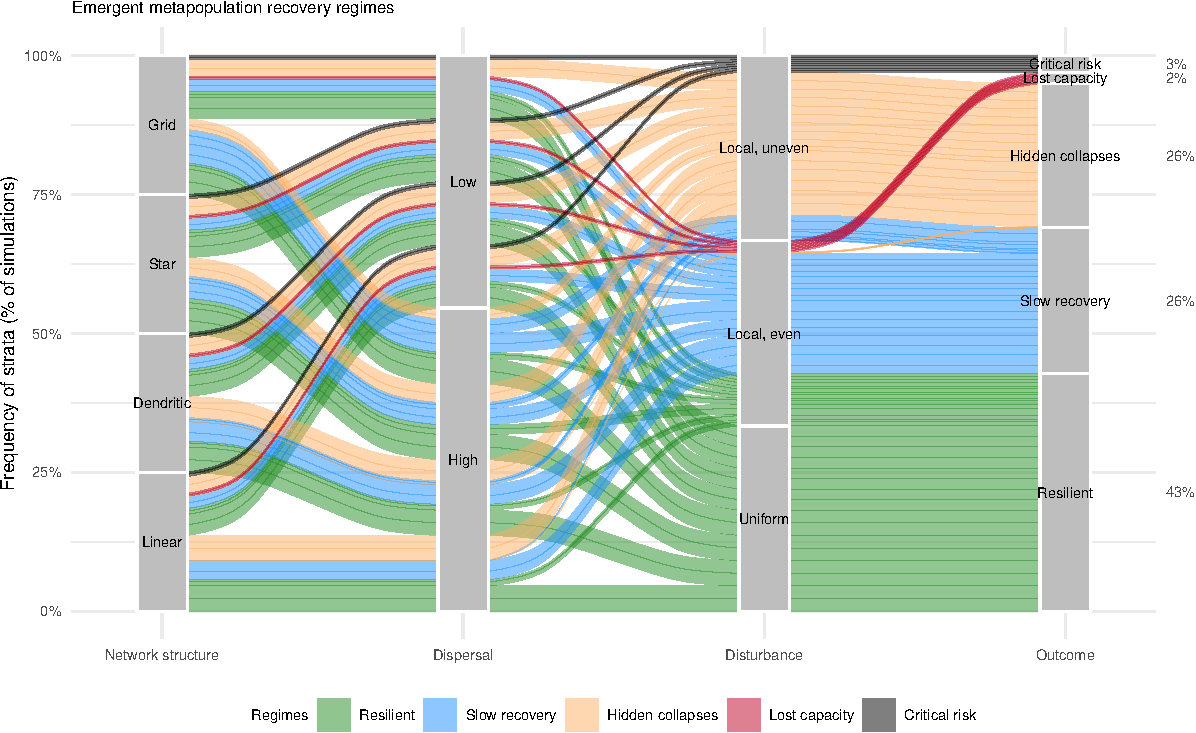
\includegraphics{Managing_for_ecological_surprises_in_metapopulations_files/figure-latex/cluster results-1} 

}

\caption{Interplay between network structure, disturbance, and dispersal can lead to suprising recovery outcomes.}\label{fig:cluster results}
\end{figure}

\hypertarget{references}{%
\subsection{References}\label{references}}

\vspace{3truemm}

\hypertarget{refs}{}
\begin{CSLReferences}{1}{0}
\leavevmode\vadjust pre{\hypertarget{ref-Anderson2015}{}}%
Anderson, S.C., Moore, J.W., McClure, M.M., Dulvy, N.K. \& Cooper, A.B.
(2015). {Portfolio conservation of metapopulations under climate
change.} \emph{Ecological Applications}, 25, 559--572.

\leavevmode\vadjust pre{\hypertarget{ref-Csardi2006}{}}%
Csardi, G. \& Nepusz, T. (2006). \href{https://igraph.org}{{The igraph
software package for complex network research}}. \emph{InterJournal},
Complex Sy, 1695.

\leavevmode\vadjust pre{\hypertarget{ref-Forrest2010}{}}%
Forrest, R.E., McAllister, M.K., Dorn, M.W., Martell, S.J.D. \& Stanley,
R.D. (2010). \href{https://doi.org/10.1139/f10-077}{{Hierarchical
Bayesian estimation of recruitment parameters and reference points for
Pacific rockfishes (Sebastes spp.) under alternative assumptions about
the stock--recruit function}}. \emph{Canadian Journal of Fisheries and
Aquatic Sciences}, 67, 1611--1634.

\leavevmode\vadjust pre{\hypertarget{ref-Moore2021}{}}%
Moore, J.W., Connors, B.M. \& Hodgson, E.E. (2021).
\href{https://doi.org/10.1111/faf.12567}{{Conservation risks and
portfolio effects in mixed‐stock fisheries}}. \emph{Fish and Fisheries},
faf.12567.

\leavevmode\vadjust pre{\hypertarget{ref-Okamoto2020}{}}%
Okamoto, D.K., Hessing‐Lewis, M., Samhouri, J.F., Shelton, A.O., Stier,
A.C., Levin, P.S. \& Salomon, A.K. (2020).
\href{https://doi.org/10.1002/eap.2051}{{Spatial variation in exploited
metapopulations obscures risk of collapse}}. \emph{Ecological
Applications}, 30, e02051.

\leavevmode\vadjust pre{\hypertarget{ref-Walters2004}{}}%
Walters, C.J. \& Martell, S.J.D. (2004). \emph{{Fisheries ecology and
management}}. Princeton University Press.

\leavevmode\vadjust pre{\hypertarget{ref-Yeakel2014}{}}%
Yeakel, J.D., Moore, J.W., Guimarães, P.R. \& Aguiar, M.A.M. de. (2014).
\href{https://doi.org/10.1111/ele.12228}{{Synchronisation and stability
in river metapopulation networks}}. \emph{Ecology Letters}, 17,
273--283.

\end{CSLReferences}

\end{document}
